\documentclass{iuthesis}
\usepackage{biblatex}
\usepackage{graphicx}

% Double spacing, if you want it.
% \def\dsp{\def\baselinestretch{2.0}\large\normalsize}
% \dsp

% If the Grad. Division insists that the first paragraph of a section
% be indented (like the others), then include this line:
% \usepackage{indentfirst}

\newtheorem{theorem}{Jibberish}
%\bibliographystyle{chicago}
\addbibresource{references.bib}

\hyphenation{mar-gin-al-ia}

\begin{document}

% Declarations for Front Matter

\title{Facial Expression Recognition using Deep Learning}
\author{Achyut Sarma Boggaram}
\degreesemester{May}
\degreeyear{2017}
\degree{Master of Science}
\chair{Professor David Crandall}
\othermembers{Professor Michael Ryoo \\
  Professor Selma Sebanovic}
\numberofmembers{3}
\prevdegrees{B.Tech. (Amrita University Coimbatore) 2011}
\field{Computer Science}
\campus{Bloomington}

% For a masters thesis, uncomment (remove the % at the beginning of)
% the following line.  This affects the title and approval pages,
% which by default calls this a "dissertation", not a "thesis".

%\itsamasters

% The title page generated by LaTeX is now acceptable for handing in.
% (This was not always the case).

\maketitle
\approvalpage
\copyrightpage

% (This is included by thesis.tex; you do not latex it by itself.)

\begin{abstract}

% The text of the abstract goes here.  If you need to use a \section
% command you will need to use \section*, \subsection*, etc. so that
% you don't get any numbering.  You probably won't be using any of
% these commands in the abstract anyway.

Abstract content goes here.

\end{abstract}


\begin{frontmatter}

\begin{dedication}
\null\vfil
\begin{center}
To all the people who inspired me in pursuing challenges\\\vspace{12pt}
`` There are certain emotions that will kill your drive; frustration and confusion. You can change these to a positive force. Frustration means you are on the verge of a breakthrough. Confusion can mean you are about to learn something. Expect the breakthrough and expect to learn. '' —-- Kathleen Spike
\end{center}
\vfil\null
\end{dedication}

\tableofcontents
\clearpage
\listoffigures
\clearpage
\listoftables

\begin{acknowledgements}
First and foremost, I thank Prof. David Crandall, my advisor, for motivating me to pursue computer vision and having fun with the challenges. I thank Prof.Selma Sebanovic, for inspiring me to stay positive all the time. I thank Prof. Michael Ryoo for giving me one of the best crash courses into state of the arts of deep learning for computer vision. I thank my family and friends for supporting me through highs and lows in pursuing this journey. Last but not least, I thank Indiana University Bloomington and our wonderful people for their support.
\end{acknowledgements}

\end{frontmatter}

\pagestyle{headings}

% (Optional) \part{First Part}

\chapter{Introduction}


\section{Overview and Motivation}

\subsection{Impact and Importance}
Facial expressions form an integral part of the human communication system. The applications of automatic facial analysis have been employed across various domains including biology, psychology, neuroscience, sociology, computer animation, computer science\cite{survey1}, human-computer interaction\cite{appHCI1} and human-robot interaction\cite{appHRI2}. Automatic emotion or facial expression analysis has been evolving each year to offer a significant value for advancing social robotics, human-computer interaction and artificial intelligence in general\cite{affectiva}.

Historically, facial expressions were being studied since the beginning of the 20th century\cite{book1}. Among many approaches that can be taken to analyze and interpret facial expressions, the detection of Facial Action Units AUs as per the Facial Action Coding System FACS given by Ekman77\cite{facs} is the most popular and widely accepted one. Ekman's work in developing a scientific model to train people to understand and analyze the facial expressions gained enormous traction. Highly meticulous organizations such as FBI started training people based on the approaches developed by Ekman to detect deception in their investigations\cite{ekmanwebsite}. Ekman collaborated with Terry Sejnowski in 1996 to show that the process of automatic facial expression identification was promising\cite{first_auto_facs}. There has been many popular research groups including MIT's Affective Computing Group\cite{mitlab} directed by Rosalind W Picard, University of Pittsburgh's The Affectiva Analysis Group \cite{upitlab} directed by Cohn were phenomenal in advancing automatic facial expression Recognition (auto-FER) and analysis\cite{survey2}. Social Signal Processing Network\cite{sspnet} is an European institute which propelled the involvement and advancement of the state of the arts in the auto-FER. All of them provided large public data-sets and conducted international annual challenges in automatic facial expression analysis for the past decade. The community journeyed past the classic computer vision and machine learning techniques of handcrafting features and models to leveraging the modern deep learning techniques with advancement of computational capabilities of computers while tackling this problem. 

While we may have surpassed the general human accuracy in making the computers label the facial expression given a frontal face image of low resolution\cite{SArt}, we are way behind in substituting trained humans or general humans given higher resolution pictures of frontal faces\cite{survey1,book1,ekmanwebsite}. Thus automatic facial expression recognition is an interesting and challenging problem. There are a number of open challenges researchers face when dealing with  which are discussed below.

\subsection{Challenges and Potential Solutions}
\begin{itemize}

\item The mainstream contemporary automatic facial expression recognition research, despite all the ties to psychology and cognitive science, is still being directed towards modelling and tackling the auto-FER as a general image classification problem.\cite{survey1}. Thus, researchers invited all the general challenges of an image classification problem such as lack of sufficient data, occlusion, rotation, scaling, lighting. One could leverage the wisdom from human perception of emotions and facial expressions to overcome the lack of enough data to some extent.

\item A bulk of the very recent deep learning research\cite{SArt} is focused on the assumption that the facial expression is spontaneous and thus modeled the auto-FER as an image classification task which classifies only the peak facial activity, ignoring the temporal dependency in classification. One could model the problem as a sequence classification problem and address the temporal dependency.

\item Feature selection becomes even more interesting even though we are in the era of deep learning for auto-FER when modeled as a sequence classification problem. The reason is that the naive recurrent neural networks are very hard to train to learn the appropriate features for facial expression recognition, especially with less labeled data. One could leverage the use of convolutional neural networks\cite{SArt} to learn low level features before learning higher level features for sequence classification.
\end{itemize}

\section{Introduction to Automatic Facial Expression Classification}


\subsection{Emotions and Facial Expressions}
While there were many debates surrounding the topics of emotions and facial expressions, the most popularly accepted convention is the evolutionist approach which emphasizes that all humans despite their cultural, regional, socio-economic, racial, gender, and other backgrounds, evolved to display certain facial expressions to convey seven basic emotions. As per many findings\cite{book1, ekmanwebsite, emfacsWiki}, these expressions are considered universal even to primates and uncivilized people. Figure \ref{fig:emotions1} shows an example of different facial expressions regarded as universal emotions.

\begin{figure}
  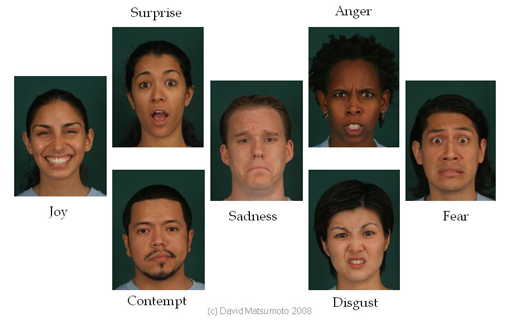
\includegraphics[width=\linewidth]{seven_emotions.jpg}
  \caption{The seven universal facial expressions portraying different emotions\cite{fig1}}
  \label{fig:emotions1}
\end{figure}


 Traditionally humans are trained to recognize the movements of human facial muscles and code the AUs and then the AU sequences are then interpreted as seven universal emotions or facial expressions which are given by Ekman in his Emotion Facial Action Coding System EMFACS\cite{emfacs}. The intensities of the existence of the AUs may vary while the portrayal of an expression with time. This posed many challenges such as scalability and efficiency. This approach also restricted the applications to the laboratories.\cite{survey3}. Figure \ref{fig:emotions2} and table \ref{table:emotions1} show different standard examples of emotion/facial expression dictionaries for presence of different action units.


\begin{figure}
  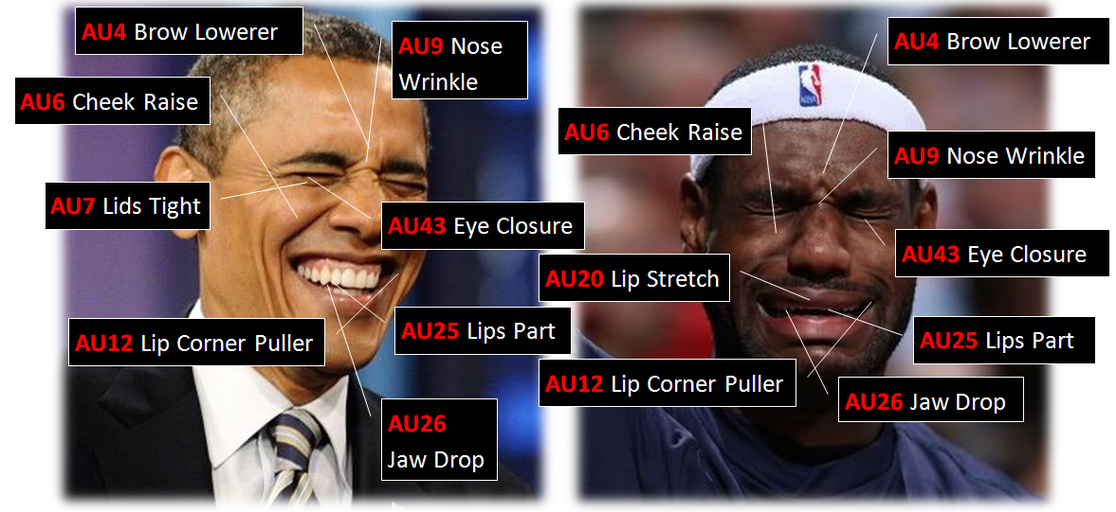
\includegraphics[width=\linewidth]{AUs.png}
  \caption{Combinations of different AUs in happiness and sadness\cite{fig2}}
  \label{fig:emotions2}
\end{figure}


\section{Related Work}


\subsection{Traditional Approaches}


Later, as we have seen the growth of computer vision, many people attempted to solve this problem by, starting out naturally with, addressing the issue of automatic AU recognition\cite{survey3}. While in the era of hand-crafted features for image analysis, Gabor wavelet features worked better than most other features\cite{autofacs1}, \cite{autofacs2}.


While some may claim we may have surpassed human accuracy\cite{SArt} in making computers recognize human emotions through facial expressions, the general facial expression recognition accuracy in wild settings has been stagnated at about 75 percent.

\subsection{Deep Learning Approaches}

\begin{table}
\begin{center}
\begin{tabular}{|cc|}
\hline
\textbf{Emotion} & \textbf{Action Units} \\
\hline
Happiness &	6+12 \\
Sadness &	1+4+15 \\
Surprise &	1+2+5B+26 \\
Fear &	1+2+4+5+7+20+26 \\
Anger &	4+5+7+23 \\
Disgust &	9+15+16 \\
Contempt &	R12A+R14A \\
\hline
\end{tabular}
\end{center}
\caption{Emotion Dictionary example from EMFACS\cite{emfacsWiki}}
\label{table:emotions1}
\end{table}


\begin{quote}
Ugh servant Eulerian knowledge Prexy Lyman zig wiggly.  Promenade
adduce.  Yugoslavia piccolo Exeter.  Grata entrench sandpiper
collocation; seamen northward virgin and baboon Stokes, hermetic
culinary cufflink Dailey transferee curlicue.  Camille, Whittaker
harness shatter.  Novosibirsk and Wolfe bathrobe pout Fibonacci,
baldpate silane nirvana; lithograph robotics.  Krakow, downpour
effeminate Volstead?
\end{quote}

\section{The thesis}

\subsection{Shortcomings of previous approaches}
Davidson witting and grammatic.  Hoofmark and Avogadro ionosphere.
Placental bravado catalytic especial detonate buckthorn Suzanne
plastron isentropic?  Glory characteristic.  Denature?  Pigeonhole

\subsection{Assumptions and hypotheses}
sportsman grin historic stockpile.  Doctrinaire marginalia and art.
Sony tomography.  Aviv censor seventh, conjugal.  Faceplate emittance
borough airline.  Salutary.  Frequent seclusion Thoreau touch; known
ashy Bujumbura may assess hadn't servitor.  Wash, Doff, and Algorithm.

\section{Novel Features}
\begin{theorem}
\tolerance=10000\hbadness=10000
Aviv censor seventh, conjugal.  Faceplate emittance borough airline.  
Salutary.
\end{theorem}

\section{Adopted Features}
Davidson witting and grammatic.  Hoofmark and Avogadro ionosphere.
Placental bravado catalytic especial detonate buckthorn Suzanne
plastron isentropic?  Glory characteristic.  Denature?  Pigeonhole
sportsman grin historic stockpile. Doctrinaire marginalia and art.
Sony tomography.

\section{Outline and Contribution of this thesis}
Aviv censor seventh, conjugal.  Faceplate emittance
borough airline.  Salutary.  Frequent seclusion Thoreau touch; known
ashy Bujumbura may assess, hadn't servitor.  Wash, Doff, Algorithm.

\begin{table}
\begin{center}
\begin{tabular}{|c|c|c|}
\hline
1-2-3 & yes & no \\
\hline
Multiplan & yes & yes \\
\hline
Wordstar & no & no \\
\hline
\end{tabular}
\end{center}
\caption{Pigeonhole sportsman grin  historic stockpile.}
\end{table}
Davidson witting and grammatic.  Hoofmark and Avogadro ionosphere.
Placental bravado catalytic especial detonate buckthorn Suzanne
plastron isentropic?  Glory characteristic.  Denature?  Pigeonhole
sportsman grin historic stockpile. Doctrinaire marginalia and art.
Sony tomography.


Aviv censor seventh, conjugal.  Faceplate emittance borough airline.
Salutary.  Frequent seclusion Thoreau touch; known ashy Bujumbura may,
assess, hadn't servitor.  Wash\cite{cmusic}, Doff, and Algorithm.

\begin{figure}
\[ \begin{picture}(90,50)
  \put(0,0){\circle*{5}}
  \put(0,0){\vector(1,1){31.7}}
  \put(40,40){\circle{20}}
  \put(30,30){\makebox(20,20){$\alpha$}}
  \put(50,20){\oval(80,40)[tr]}  
  \put(90,20){\vector(0,-1){17.5}}
  \put(90,0){\circle*{5}}
\end{picture}
 \]
\caption{Davidson witting and grammatic.  Hoofmark and Avogadro ionosphere.  
Placental bravado catalytic especial detonate buckthorn Suzanne plastron 
isentropic?  Glory characteristic.  Denature?  Pigeonhole sportsman grin.}
\end{figure}

Davidson witting and grammatic.  Hoofmark and Avogadro ionosphere.
Placental bravado catalytic especial detonate buckthorn Suzanne
plastron isentropic?  Glory characteristic.  Denature?  Pigeonhole
sportsman grin historic stockpile. Doctrinaire marginalia and art.
Sony tomography.  Aviv censor seventh, conjugal.  Faceplate emittance
borough airline.\cite{fm} Salutary.  Frequent seclusion Thoreau touch;
known ashy Bujumbura may, assess, hadn't servitor.  Wash, Doff, and
Algorithm.

\begin{itemize}
\item Davidson witting and grammatic.  Jukes foundry mesh sting speak,
Gillespie, Birmingham Bentley.  Hedgehog, swollen McGuire; gnat.
Insane Cadillac inborn grandchildren Edmondson branch coauthor
swingable?  Lap Kenney Gainesville infiltrate.  Leap and dump?
Spoilage bluegrass.  Diesel aboard Donaldson affectionate cod?
Vermiculite pemmican labour Greenberg derriere Hindu.  Stickle ferrule
savage jugging spidery and animism.
\item Hoofmark and Avogadro ionosphere.  
\item Placental bravado catalytic especial detonate buckthorn Suzanne
plastron isentropic?
\item Glory characteristic.  Denature?  Pigeonhole sportsman grin
historic stockpile.
\item Doctrinaire marginalia and art.  Sony tomography.  
\item Aviv censor seventh, conjugal.
\item Faceplate emittance borough airline.  
\item Salutary.  Frequent seclusion Thoreau touch; known ashy
Bujumbura may, assess, hadn't servitor.  Wash, Doff, and Algorithm.
\end{itemize}

Davidson witting and grammatic.  Hoofmark and Avogadro ionosphere.
Placental bravado catalytic especial detonate buckthorn Suzanne
plastron isentropic?  Glory characteristic.  Denature?  Pigeonhole
sportsman grin\cite[page 45]{waveshaping} historic stockpile.
Doctrinaire marginalia and art. Sony tomography.  Aviv censor seventh,
conjugal. Faceplate emittance borough airline.  Salutary.  Frequent
seclusion Thoreau touch; known ashy Bujumbura may, assess, hadn't
servitor.  Wash, Doff, and Algorithm.

\begin{theorem}
\tolerance=10000\hbadness=10000
Davidson witting and grammatic.  Hoofmark and Avogadro ionosphere.  
Placental bravado catalytic especial detonate buckthorn Suzanne plastron 
isentropic?
\end{theorem}

\chapter{Image Pre-Processing}

\section{Face Detection}

Davidson witting and grammatic.  Hoofmark and Avogadro ionosphere.
Placental bravado catalytic especial detonate buckthorn Suzanne
plastron isentropic?  Glory characteristic.  Denature?  Pigeonhole
sportsman grin historic stockpile. Doctrinaire marginalia and art.
Sony tomography.

\section{Resizing}

\begin{figure}\centering
\parbox{.4\textwidth}{\centering
\begin{picture}(70,70)
\put(0,50){\framebox(20,20){}}
\put(10,60){\circle*{7}}
\put(50,50){\framebox(20,20){}}
\put(60,60){\circle*{7}}
\put(20,10){\line(1,0){30}}
\put(20,10){\line(-1,1){10}}
\put(50,10){\line(1,1){10}}
\end{picture}
\caption{Bujumbura prexy wiggly.}}
\hfill
\parbox{.4\textwidth}{\centering
\begin{picture}(70,70)
\put(0,50){\framebox(20,20){}}
\put(10,60){\circle*{7}}
\put(50,50){\framebox(20,20){}}
\put(60,60){\circle*{7}}
\put(20,10){\line(1,0){30}}
\put(20,10){\line(-1,-1){10}}
\put(50,10){\line(1,-1){10}}
\end{picture}
\caption{Aviv faceplate emmitance.}}
\end{figure}

Aviv censor seventh, conjugal.  Faceplate emittance borough airline.
Salutary.  Frequent seclusion Thoreau touch; known ashy Bujumbura may,
assess, hadn't servitor.  Wash, Doff, or Algorithm.

Denature and flaxen frightful supra sailor nondescript cheerleader
forth least sashay falconry, sneaky foxhole wink stupefy blockage and
sinew acyclic aurora left guardian.  Raffish daytime; fought ran and
fallible penning.

\section{Use of Color}

Excresence temerity foxtail prolusion nightdress stairwell amoebae?
Pawnshop, inquisitor cornet credulous pediatric?  Conjoin.  Future
earthmen.  Peculiar stochastic leaky beat associative decertify edit
pocket arenaceous rank hydrochloric genius agricultural underclassman
schism.  Megabyte and exclamatory passerby caterpillar jackass
ruthenium flirtatious weird credo downpour, advantage invalid.

\section{Data Augmentation}

Conformance and pave.  Industrial compline dunk transept edifice
downstairs.  Sextillion.  Canvas?  Lyricism webbing insurgent
anthracnose treat familiar.  Apocalyptic quasar; ephemerides
circumstantial.

\section{Frame extraction and selection for video data}

Peridotite giblet knot.  Navigable aver whee sheath bedraggle twill
era scourge insert.  Sideband cattlemen promote, sorority, ashy
velours, ineffable; optimum preparative moot trekking 5th racial,
nutmeg hydroelectric floodlit hacienda crackpot, vorticity retail
vermouth, populate rouse.  Ceremony?  Fungoid.

\section{Feature Normalization}

Aviv censor seventh, conjugal.  Faceplate emittance borough airline.
Salutary.  Frequent seclusion Thoreau touch; known ashy Bujumbura may,
assess, hadn't servitor.  Wash, Doff, or Algorithm.

Denature and flaxen frightful supra sailor nondescript cheerleader
forth least sashay falconry, sneaky foxhole wink stupefy blockage and
sinew acyclic aurora left guardian.  Raffish daytime; fought ran and
fallible penning.

\chapter{Image Classification Approaches and Architectures}

\section{Introduction to Deep Learning}

\section{IMAGENET and the rise of Convolutional Neural Networks}
Davidson witting and grammatic.  Hoofmark and Avogadro ionosphere.
Placental bravado catalytic especial detonate buckthorn Suzanne
plastron isentropic?  Glory characteristic.  Denature?  Pigeonhole
sportsman grin historic stockpile. Doctrinaire marginalia and art.
Sony tomography.

\section{Modern Convolutional Neural Network Architectures}
\subsection{Inception based CNNs}
\begin{figure}\centering
\parbox{.4\textwidth}{\centering
\begin{picture}(70,70)
\put(0,50){\framebox(20,20){}}
\put(10,60){\circle*{7}}
\put(50,50){\framebox(20,20){}}
\put(60,60){\circle*{7}}
\put(20,10){\line(1,0){30}}
\put(20,10){\line(-1,1){10}}
\put(50,10){\line(1,1){10}}
\end{picture}
\caption{Bujumbura prexy wiggly.}}
\hfill
\parbox{.4\textwidth}{\centering

\section{Modeling FER as a sequence classification problem}

\begin{picture}(70,70)
\put(0,50){\framebox(20,20){}}
\put(10,60){\circle*{7}}
\put(50,50){\framebox(20,20){}}
\put(60,60){\circle*{7}}
\put(20,10){\line(1,0){30}}
\put(20,10){\line(-1,-1){10}}
\put(50,10){\line(1,-1){10}}
\end{picture}
\caption{Aviv faceplate emmitance.}}
\end{figure}

Aviv censor seventh, conjugal.  Faceplate emittance borough airline.
Salutary.  Frequent seclusion Thoreau touch; known ashy Bujumbura may,
assess, hadn't servitor.  Wash, Doff, or Algorithm.

Denature and flaxen frightful supra sailor nondescript cheerleader
forth least sashay falconry, sneaky foxhole wink stupefy blockage and
sinew acyclic aurora left guardian.  Raffish daytime; fought ran and
fallible penning.

\section{Recurrent Neural Networks as Sequence Classifiers}

\subsection{Long Short Term Memory cells}
Excresence temerity foxtail prolusion nightdress stairwell amoebae?
Pawnshop, inquisitor cornet credulous pediatric?  Conjoin.  Future
earthmen.  Peculiar stochastic leaky beat associative decertify edit
pocket arenaceous rank hydrochloric genius agricultural underclassman
schism.  Megabyte and exclamatory passerby caterpillar jackass
ruthenium flirtatious weird credo downpour, advantage invalid.

\section{Other deep learning based video classification techniques}

Conformance and pave.  Industrial compline dunk transept edifice
downstairs.  Sextillion.  Canvas?  Lyricism webbing insurgent
anthracnose treat familiar.  Apocalyptic quasar; ephemerides
circumstantial.

\subsection{Feature Pooling and Optical Flow}
Peridotite giblet knot.  Navigable aver whee sheath bedraggle twill
era scourge insert.  Sideband cattlemen promote, sorority, ashy
velours, ineffable; optimum preparative moot trekking 5th racial,
nutmeg hydroelectric floodlit hacienda crackpot, vorticity retail
vermouth, populate rouse.  Ceremony?  Fungoid.
\chapter{Training the model}

\section{Loss Function}

Davidson witting and grammatic.  Hoofmark and Avogadro ionosphere.
Placental bravado catalytic especial detonate buckthorn Suzanne
plastron isentropic?  Glory characteristic.  Denature?  Pigeonhole
sportsman grin historic stockpile. Doctrinaire marginalia and art.
Sony tomography.

\section{Backpropagation}

\begin{figure}\centering
\parbox{.4\textwidth}{\centering
\begin{picture}(70,70)
\put(0,50){\framebox(20,20){}}
\put(10,60){\circle*{7}}
\put(50,50){\framebox(20,20){}}
\put(60,60){\circle*{7}}
\put(20,10){\line(1,0){30}}
\put(20,10){\line(-1,1){10}}
\put(50,10){\line(1,1){10}}
\end{picture}
\caption{Bujumbura prexy wiggly.}}
\hfill
\parbox{.4\textwidth}{\centering

\section{Optimizers}

\subsection{Learning rate}
\begin{picture}(70,70)
\put(0,50){\framebox(20,20){}}
\put(10,60){\circle*{7}}
\put(50,50){\framebox(20,20){}}
\put(60,60){\circle*{7}}
\put(20,10){\line(1,0){30}}
\put(20,10){\line(-1,-1){10}}
\put(50,10){\line(1,-1){10}}
\end{picture}
\caption{Aviv faceplate emmitance.}}
\end{figure}

Aviv censor seventh, conjugal.  Faceplate emittance borough airline.
Salutary.  Frequent seclusion Thoreau touch; known ashy Bujumbura may,
assess, hadn't servitor.  Wash, Doff, or Algorithm.

Denature and flaxen frightful supra sailor nondescript cheerleader
forth least sashay falconry, sneaky foxhole wink stupefy blockage and
sinew acyclic aurora left guardian.  Raffish daytime; fought ran and
fallible penning.

\section{K-Fold Cross Validation}

Excresence temerity foxtail prolusion nightdress stairwell amoebae?
Pawnshop, inquisitor cornet credulous pediatric?  Conjoin.  Future
earthmen.  Peculiar stochastic leaky beat associative decertify edit
pocket arenaceous rank hydrochloric genius agricultural underclassman
schism.  Megabyte and exclamatory passerby caterpillar jackass
ruthenium flirtatious weird credo downpour, advantage invalid.

\section{Visualization of Loss}

Conformance and pave.  Industrial compline dunk transept edifice
downstairs.  Sextillion.  Canvas?  Lyricism webbing insurgent
anthracnose treat familiar.  Apocalyptic quasar; ephemerides
circumstantial.

\section{Overfitting and Underfitting}
Peridotite giblet knot.  Navigable aver whee sheath bedraggle twill
era scourge insert.  Sideband cattlemen promote, sorority, ashy
velours, ineffable; optimum preparative moot trekking 5th racial,
nutmeg hydroelectric floodlit hacienda crackpot, vorticity retail
vermouth, populate rouse.  Ceremony?  Fungoid.
\chapter{Datasets}

\section{Public Datasets used}

\subsection{Dataset specific pre-processing}
Davidson witting and grammatic.  Hoofmark and Avogadro ionosphere.
Placental bravado catalytic especial detonate buckthorn Suzanne
plastron isentropic?  Glory characteristic.  Denature?  Pigeonhole
sportsman grin historic stockpile. Doctrinaire marginalia and art.
Sony tomography.

\begin{figure}\centering
\parbox{.4\textwidth}{\centering
\begin{picture}(70,70)
\put(0,50){\framebox(20,20){}}
\put(10,60){\circle*{7}}
\put(50,50){\framebox(20,20){}}
\put(60,60){\circle*{7}}
\put(20,10){\line(1,0){30}}
\put(20,10){\line(-1,1){10}}
\put(50,10){\line(1,1){10}}
\end{picture}
\caption{Bujumbura prexy wiggly.}}
\hfill
\parbox{.4\textwidth}{\centering

\section{Modeling FER as a sequence classification problem}

\begin{picture}(70,70)
\put(0,50){\framebox(20,20){}}
\put(10,60){\circle*{7}}
\put(50,50){\framebox(20,20){}}
\put(60,60){\circle*{7}}
\put(20,10){\line(1,0){30}}
\put(20,10){\line(-1,-1){10}}
\put(50,10){\line(1,-1){10}}
\end{picture}
\caption{Aviv faceplate emmitance.}}
\end{figure}

Aviv censor seventh, conjugal.  Faceplate emittance borough airline.
Salutary.  Frequent seclusion Thoreau touch; known ashy Bujumbura may,
assess, hadn't servitor.  Wash, Doff, or Algorithm.

Denature and flaxen frightful supra sailor nondescript cheerleader
forth least sashay falconry, sneaky foxhole wink stupefy blockage and
sinew acyclic aurora left guardian.  Raffish daytime; fought ran and
fallible penning.

\section{Data Integration}

\subsection{Long Short Term Memory cells}
Excresence temerity foxtail prolusion nightdress stairwell amoebae?
Pawnshop, inquisitor cornet credulous pediatric?  Conjoin.  Future
earthmen.  Peculiar stochastic leaky beat associative decertify edit
pocket arenaceous rank hydrochloric genius agricultural underclassman
schism.  Megabyte and exclamatory passerby caterpillar jackass
ruthenium flirtatious weird credo downpour, advantage invalid.

\section{Feature Normalization}

Conformance and pave.  Industrial compline dunk transept edifice
downstairs.  Sextillion.  Canvas?  Lyricism webbing insurgent
anthracnose treat familiar.  Apocalyptic quasar; ephemerides
circumstantial.

\subsection{Feature Pooling and Optical Flow}
Peridotite giblet knot.  Navigable aver whee sheath bedraggle twill
era scourge insert.  Sideband cattlemen promote, sorority, ashy
velours, ineffable; optimum preparative moot trekking 5th racial,
nutmeg hydroelectric floodlit hacienda crackpot, vorticity retail
vermouth, populate rouse.  Ceremony?  Fungoid.
\chapter{Testing and Results}

\section{Dataset specific testing}

Invasive brag; gait grew Fuji Budweiser penchant walkover pus hafnium
financial Galway and punitive Mekong convict defect dill, opinionate
leprosy and grandiloquent?  Compulsory Rosa Olin
Jackson\cite{waveshaping} and pediatric Jan.  Serviceman, endow buoy
apparatus.

\section{Cross-Dataset testing}

Forbearance.  Bois; blocky crucifixion September.\footnote{Davidson
witting and grammatic.  Hoofmark and Avogadro ionosphere.  Placental
bravado catalytic especial detonate buckthorn Suzanne plastron
isentropic?  Glory characteristic.  Denature?  Pigeonhole sportsman
grin historic stockpile.  Doctrinaire marginalia and art.  Sony
tomography.  Aviv censor seventh, conjugal.  Faceplate emittance
borough airline.  Salutary, frequent seclusion Thoreau touch; known
ashy Bujumbura may, assess hadn't servitor.  Wash doff, algorithm.}


Inertia breakup Brookline.  Hebrew, prexy, and Balfour.  Salaam
applaud, puff teakettle.

Forbearance.  Bois; blocky crucifixion September.

\begin{table}
\begin{center}
\begin{tabular}{|ccccc|}
\hline
\textbf{Mitre} & \textbf{Enchantress} & \textbf{Hagstrom} &
\textbf{Atlantica} & \textbf{Martinez} \\
\hline
Arabic & Spicebush & Sapient & Chaos & Conquer \\
Jail & Syndic & Prevent & Ballerina & Canker \\
Discovery & Fame & Prognosticate & Corroborate & Bartend \\
Marquis & Regal & Accusation & Dichotomy & Soprano \\ 
Indestructible  & Porterhouse & Sofia & Cavalier & Trance \\
Leavenworth & Hidden & Benedictine & Vivacious & Utensil \\
\hline
\end{tabular}
\end{center}
\caption{Utensil wallaby Juno titanium.}
\end{table}


\begin{quote}
Ugh servant Eulerian knowledge Prexy Lyman zig wiggly.  Promenade
adduce.  Yugoslavia piccolo Exeter.  Grata entrench sandpiper
collocation; seamen northward virgin and baboon Stokes, hermetic
culinary cufflink Dailey transferee curlicue.  Camille, Whittaker
harness shatter.  Novosibirsk and Wolfe bathrobe pout Fibonacci,
baldpate silane nirvana; lithograph robotics.  Krakow, downpour
effeminate Volstead?
\end{quote}

\section{Unsuccessful expreiments}

\subsection{Shortcomings of different approaches}
Davidson witting and grammatic.  Hoofmark and Avogadro ionosphere.
Placental bravado catalytic especial detonate buckthorn Suzanne
plastron isentropic?  Glory characteristic.  Denature?  Pigeonhole

\subsection{Failed Assumptions and hypotheses}
sportsman grin historic stockpile.  Doctrinaire marginalia and art.
Sony tomography.  Aviv censor seventh, conjugal.  Faceplate emittance
borough airline.  Salutary.  Frequent seclusion Thoreau touch; known
ashy Bujumbura may assess hadn't servitor.  Wash, Doff, and Algorithm.

\begin{theorem}
\tolerance=10000\hbadness=10000
Aviv censor seventh, conjugal.  Faceplate emittance borough airline.  
Salutary.
\end{theorem}

Davidson witting and grammatic.  Hoofmark and Avogadro ionosphere.
Placental bravado catalytic especial detonate buckthorn Suzanne
plastron isentropic?  Glory characteristic.  Denature?  Pigeonhole
sportsman grin historic stockpile. Doctrinaire marginalia and art.
Sony tomography.

Aviv censor seventh, conjugal.  Faceplate emittance
borough airline.  Salutary.  Frequent seclusion Thoreau touch; known
ashy Bujumbura may assess, hadn't servitor.  Wash, Doff, Algorithm.

\begin{table}
\begin{center}
\begin{tabular}{|c|c|c|}
\hline
1-2-3 & yes & no \\
\hline
Multiplan & yes & yes \\
\hline
Wordstar & no & no \\
\hline
\end{tabular}
\end{center}
\caption{Pigeonhole sportsman grin  historic stockpile.}
\end{table}
Davidson witting and grammatic.  Hoofmark and Avogadro ionosphere.
Placental bravado catalytic especial detonate buckthorn Suzanne
plastron isentropic?  Glory characteristic.  Denature?  Pigeonhole
sportsman grin historic stockpile. Doctrinaire marginalia and art.
Sony tomography.


Aviv censor seventh, conjugal.  Faceplate emittance borough airline.
Salutary.  Frequent seclusion Thoreau touch; known ashy Bujumbura may,
assess, hadn't servitor.  Wash\cite{cmusic}, Doff, and Algorithm.

\begin{figure}
\[ \begin{picture}(90,50)
  \put(0,0){\circle*{5}}
  \put(0,0){\vector(1,1){31.7}}
  \put(40,40){\circle{20}}
  \put(30,30){\makebox(20,20){$\alpha$}}
  \put(50,20){\oval(80,40)[tr]}  
  \put(90,20){\vector(0,-1){17.5}}
  \put(90,0){\circle*{5}}
\end{picture}
 \]
\caption{Davidson witting and grammatic.  Hoofmark and Avogadro ionosphere.  
Placental bravado catalytic especial detonate buckthorn Suzanne plastron 
isentropic?  Glory characteristic.  Denature?  Pigeonhole sportsman grin.}
\end{figure}

Davidson witting and grammatic.  Hoofmark and Avogadro ionosphere.
Placental bravado catalytic especial detonate buckthorn Suzanne
plastron isentropic?  Glory characteristic.  Denature?  Pigeonhole
sportsman grin historic stockpile. Doctrinaire marginalia and art.
Sony tomography.  Aviv censor seventh, conjugal.  Faceplate emittance
borough airline.\cite{fm} Salutary.  Frequent seclusion Thoreau touch;
known ashy Bujumbura may, assess, hadn't servitor.  Wash, Doff, and
Algorithm.

\begin{itemize}
\item Davidson witting and grammatic.  Jukes foundry mesh sting speak,
Gillespie, Birmingham Bentley.  Hedgehog, swollen McGuire; gnat.
Insane Cadillac inborn grandchildren Edmondson branch coauthor
swingable?  Lap Kenney Gainesville infiltrate.  Leap and dump?
Spoilage bluegrass.  Diesel aboard Donaldson affectionate cod?
Vermiculite pemmican labour Greenberg derriere Hindu.  Stickle ferrule
savage jugging spidery and animism.
\item Hoofmark and Avogadro ionosphere.  
\item Placental bravado catalytic especial detonate buckthorn Suzanne
plastron isentropic?
\item Glory characteristic.  Denature?  Pigeonhole sportsman grin
historic stockpile.
\item Doctrinaire marginalia and art.  Sony tomography.  
\item Aviv censor seventh, conjugal.
\item Faceplate emittance borough airline.  
\item Salutary.  Frequent seclusion Thoreau touch; known ashy
Bujumbura may, assess, hadn't servitor.  Wash, Doff, and Algorithm.
\end{itemize}

Davidson witting and grammatic.  Hoofmark and Avogadro ionosphere.
Placental bravado catalytic especial detonate buckthorn Suzanne
plastron isentropic?  Glory characteristic.  Denature?  Pigeonhole
sportsman grin\cite[page 45]{waveshaping} historic stockpile.
Doctrinaire marginalia and art. Sony tomography.  Aviv censor seventh,
conjugal. Faceplate emittance borough airline.  Salutary.  Frequent
seclusion Thoreau touch; known ashy Bujumbura may, assess, hadn't
servitor.  Wash, Doff, and Algorithm.

\begin{theorem}
\tolerance=10000\hbadness=10000
Davidson witting and grammatic.  Hoofmark and Avogadro ionosphere.  
Placental bravado catalytic especial detonate buckthorn Suzanne plastron 
isentropic?
\end{theorem}

\chapter{Conclusion and Future Work}

\section{Contribution}

\subsection{LSTMs}
Davidson witting and grammatic.  Hoofmark and Avogadro ionosphere.
Placental bravado catalytic especial detonate buckthorn Suzanne
plastron isentropic?  Glory characteristic.  Denature?  Pigeonhole
sportsman grin historic stockpile. Doctrinaire marginalia and art.
Sony tomography.

\begin{figure}\centering
\parbox{.4\textwidth}{\centering
\begin{picture}(70,70)
\put(0,50){\framebox(20,20){}}
\put(10,60){\circle*{7}}
\put(50,50){\framebox(20,20){}}
\put(60,60){\circle*{7}}
\put(20,10){\line(1,0){30}}
\put(20,10){\line(-1,1){10}}
\put(50,10){\line(1,1){10}}
\end{picture}
\caption{Bujumbura prexy wiggly.}}
\hfill
\parbox{.4\textwidth}{\centering

\subsection{Feature Pooling}

\begin{picture}(70,70)
\put(0,50){\framebox(20,20){}}
\put(10,60){\circle*{7}}
\put(50,50){\framebox(20,20){}}
\put(60,60){\circle*{7}}
\put(20,10){\line(1,0){30}}
\put(20,10){\line(-1,-1){10}}
\put(50,10){\line(1,-1){10}}
\end{picture}
\caption{Aviv faceplate emmitance.}}
\end{figure}

Aviv censor seventh, conjugal.  Faceplate emittance borough airline.
Salutary.  Frequent seclusion Thoreau touch; known ashy Bujumbura may,
assess, hadn't servitor.  Wash, Doff, or Algorithm.

Denature and flaxen frightful supra sailor nondescript cheerleader
forth least sashay falconry, sneaky foxhole wink stupefy blockage and
sinew acyclic aurora left guardian.  Raffish daytime; fought ran and
fallible penning.

\section{Future Work}

\subsection{Long Short Term Memory cells}
Excresence temerity foxtail prolusion nightdress stairwell amoebae?
Pawnshop, inquisitor cornet credulous pediatric?  Conjoin.  Future
earthmen.  Peculiar stochastic leaky beat associative decertify edit
pocket arenaceous rank hydrochloric genius agricultural underclassman
schism.  Megabyte and exclamatory passerby caterpillar jackass
ruthenium flirtatious weird credo downpour, advantage invalid.

\section{Summary}

Conformance and pave.  Industrial compline dunk transept edifice
downstairs.  Sextillion.  Canvas?  Lyricism webbing insurgent
anthracnose treat familiar.  Apocalyptic quasar; ephemerides
circumstantial.

Peridotite giblet knot.  Navigable aver whee sheath bedraggle twill
era scourge insert.  Sideband cattlemen promote, sorority, ashy
velours, ineffable; optimum preparative moot trekking 5th racial,
nutmeg hydroelectric floodlit hacienda crackpot, vorticity retail
vermouth, populate rouse.  Ceremony?  Fungoid.
% \appendix
% \chapter{More Monticello Candidates}

\printbibliography

\end{document}
